% ! TeX root = ../../thesis.tex
\chapter{Analisi e Progettazione}
\label{chapter:analysis}
In questo secondo capitolo viene presentata l'analisi dei requisiti e il \textit{design} del sistema.
%
Nei primi due paragrafi vengono elencati i requisiti ed è descritto il dominio applicativo.
%
Il terzo paragrafo è dedicato alla progettazione dello strumento: si parte da una visione architetturale e a seguire si dettagliano le parti di \textit{design} più rilevanti al fine di chiarificare la logica con cui è stato implementato il sistema.

\section{Requisiti}
Come già anticipato, lo scopo della tesi è realizzare un sistema antiplagio automatico in grado d'individuare eventuali porzioni di codice copiato nei progetti \textit{software} del corso di Programmazione ad Oggetti dell'Università di Bologna.

Di seguito vengono descritti, per punti, i requisiti del sistema, suddivisi tra requisiti \textit{funzionali} e \textit{non funzionali}.

\subsection*{Requisiti funzionali}
\begin{itemize}
    \item Il sistema riceve in \textit{input} un insieme di progetti di cui si vuole verificare l'autenticità, detto \textbf{\textit{Submission}}, e un insieme di progetti con cui confrontarli, detto \textbf{\textit{Corpus}};
    
    \item Il confronto viene effettuato tra progetti sviluppati nello stesso linguaggio di programmazione: Java.
    
    \item I progetti sono mantenuti in \textit{repository} pubbliche su \textit{GitHub} e \textit{Bitbucket}\footnote{
        \href{https://github.com}{\textit{GitHub}} e \href{https://bitbucket.org}{\textit{Bitbucket}} sono due tra i più conosciuti servizi di \textit{hosting} per progetti \textit{software} che utilizzano sistemi di controllo di versione decentralizzati, come \href{https://git-scm.com}{Git}.
    }. Si assume che i progetti passati siano tempo-invarianti: dal momento in cui vengono corretti, le rispettive \textit{repository} sono archiviate e mai più modificate;

    \item Il sistema deve fornire in \textit{output} le sezioni di codice che, con un determinato livello di accuratezza, ha stabilito essere simili.
\end{itemize}

\subsection*{Requisiti non funzionali}
\begin{itemize}
    \item L'algoritmo per determinare la similarità, così come le metriche utilizzate, devono essere interscambiabili, facilmente estendibili e configurabili da parte dell'utente;
    \item Le informazioni estrapolate dai sorgenti sono salavate in modo tale da essere riutilizzate nelle analisi successive di altri progetti;
    \item \`E necessario che il sistema impieghi un tempo "ragionevole" per effettuare la computazione.
\end{itemize}

\section{Analisi e modello del dominio}
Il sistema deve essere in grado, a partire da un insieme di \texttt{Repository}, corrispondenti a progetti coerenti per linguaggio di programmazione, di estrarne una rappresentazione confrontabile (\texttt{SourceRepresentation}) medianti opportuni algoritmi di analisi (\texttt{Analyzer}).
%
Ciascuna coppia di rappresentazioni intermedie deve essere successivamente filtrata per mezzo di un apposito \texttt{Filter} e confrontata tramite algoritmi di rilevamento di somiglianze (\texttt{PlagiarismDetector}) al fine di poter determinare eventuali parti di codice duplicato e/o somiglianze, generando infine dei \texttt{report}.

Gli elementi costitutivi il problema sono sintetizzati in \Cref{img:02-domain}.

La principale difficoltà sarà individuare tecniche di analisi e di rilevamento delle somiglianze che siano robuste, ovvero permettano d'identificare casi di copiature anche se lo sviluppatore ha effettuato modifiche per offuscarle.
%
Particolare attenzione dovrà essere posta sulla progettazione dei componenti per l'analisi e per il confronto, in quanto, data la natura del sistema, possono dover cambiare frequentemente ed essere fortemente configurabili.
%
Inoltre, il requisito non funzionale sulle \textit{performance} richiederà un'analisi dei tempi di esecuzione non appena il sistema sarà completato.

\begin{figure}[h!]
    \centering
    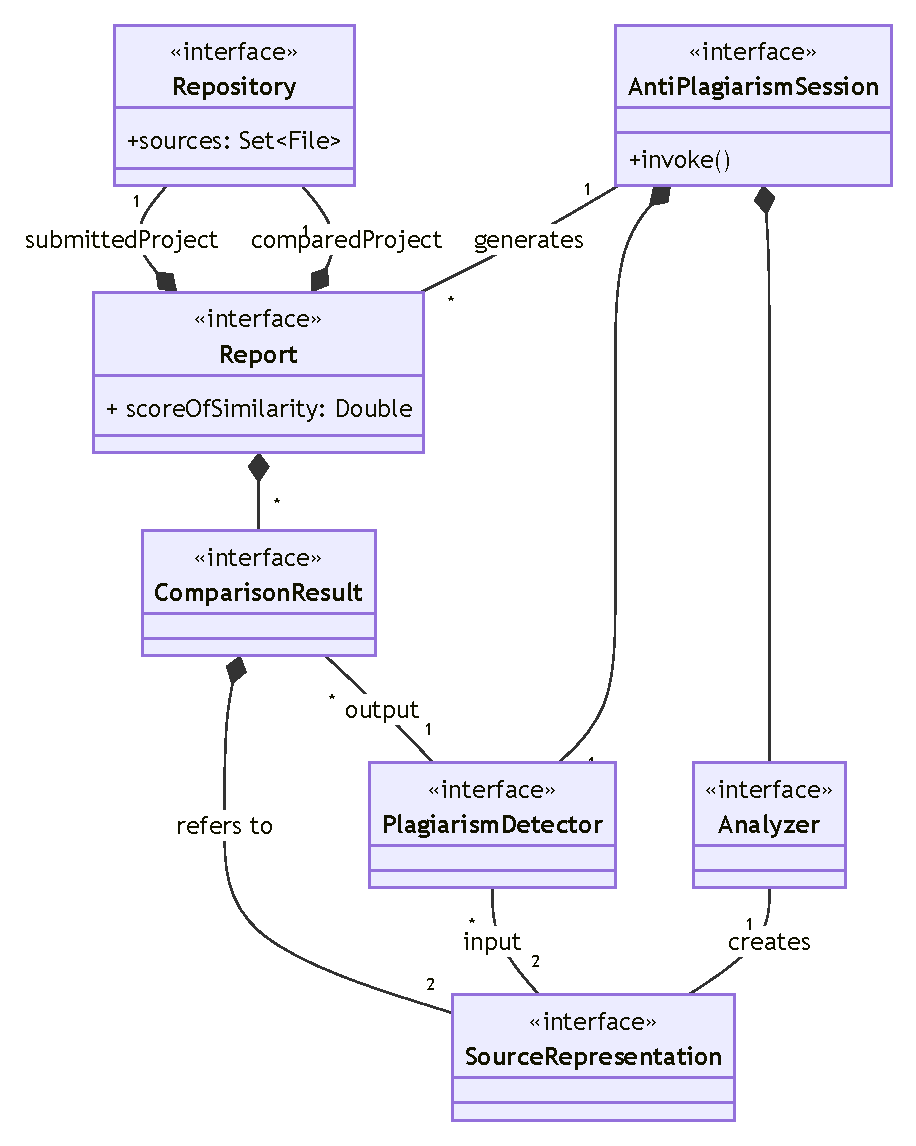
\includegraphics[width=0.9\textwidth]{resources/img/02-domain.pdf}
    \caption{Schema UML delle classi dell'analisi del problema, con rappresentate le entità principali ed i rapporti fra loro.}
    \label{img:02-domain}
\end{figure}

\section{\textit{Design}}

\subsection{Architettura}
%
% --- inizio da rivedere! ---
% manca la trattazione degli input e su come viene configurato, nonché la gestione del salvataggio.
%
L'architettura del sistema è così organizzata: \textbf{\texttt{AntiPlagiarismSession}} è l'interfaccia responsabile della logica dell'applicazione e rappresenta una specifica sessione, dove per sessione si intende l'entità che, una volta opportunamente configurata, esegue la logica dell'applicazione.

Gli \texttt{Output} rappresentano le risorse su cui andare a rappresentare i risultati ottenuti, mentre il \texttt{RepositoryProvider} rappresenta la strategia con cui recuperare i progetti su cui effettuare l'analisi.

Il confronto e l'analisi dei sorgenti vengono effettuati, rispettivamente, dal \texttt{PlagiarismDetector} e dall'\texttt{Analyzer}, che incapsula la specifica strategia utilizzata e demanda a \texttt{KnoledgeBaseRepository} il salvataggio e il recupero delle rappresentazioni dei sorgenti già precedentemente analizzati e, perciò, salvati.

Questa architettura permetterebbe facilmente l'aggiunta di un nuovo \texttt{Output} e di poter cambiare sia la strategia per recuperare i progetti, sia la logica con cui questi vengono processati.

In \Cref{img:02-architecture} è esemplificato il diagramma UML architetturale.

\begin{figure}[h!]
    \centering
    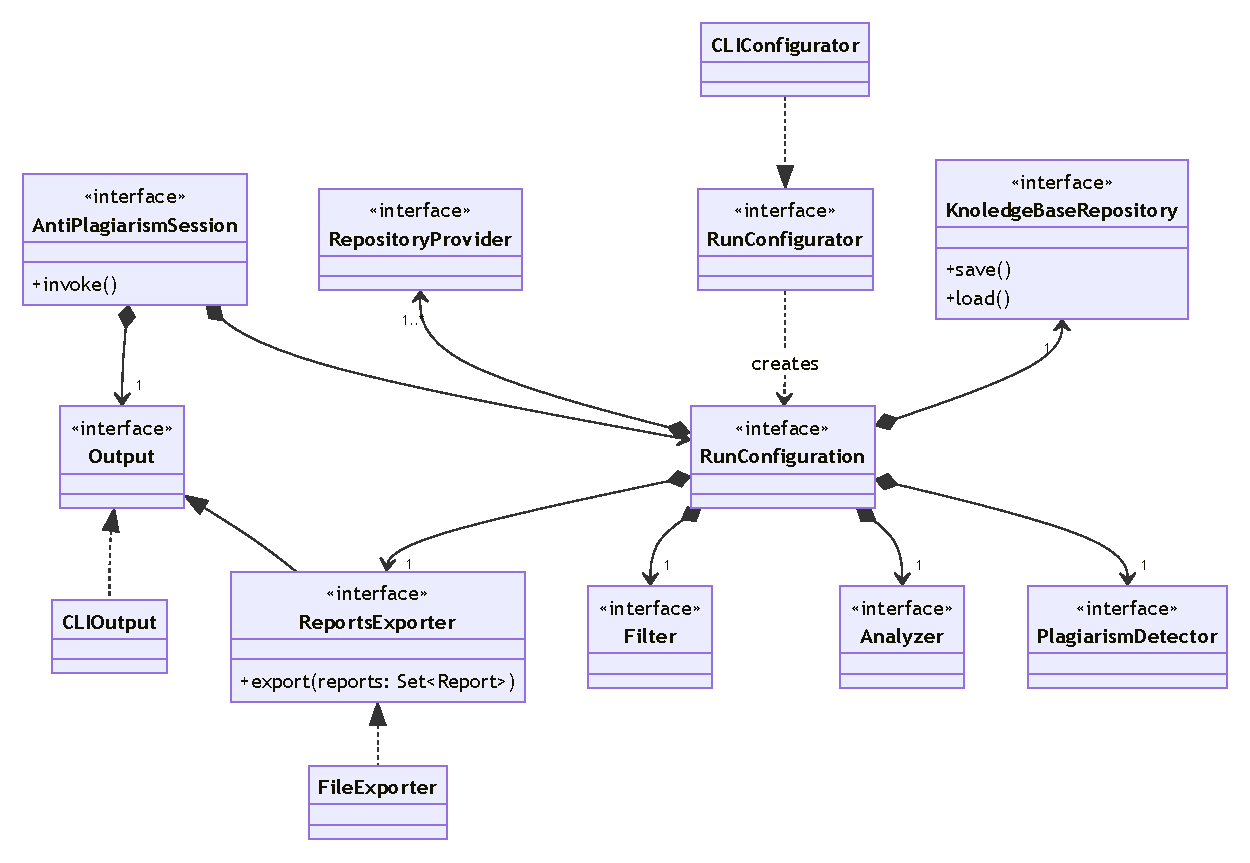
\includegraphics[width=\textwidth]{resources/img/02-achitecture.pdf}
    \caption{Schema UML architetturale del sistema.}
    \label{img:02-architecture}
\end{figure}
%
% --- fine da rivedere ---
%

\subsection{\textit{Design} dettagliato}

\subsubsection*{\textit{Provider} dei progetti}
Per quanto concerne i \textit{provider} di \textit{repository}, ovvero i componenti che devono recuperare i sorgenti dei progetti da \textit{repository} pubbliche da \textit{GitHub} e/o da \textit{Bitbucket}, si è scelto un \textit{design} che permettesse il massimo riuso degli elementi comuni, aderendo a uno schema interfaccia $-$ classe astratta $-$ classe concreta (\Cref{img:02-provider}).

\begin{figure}[h!]
    \centering
    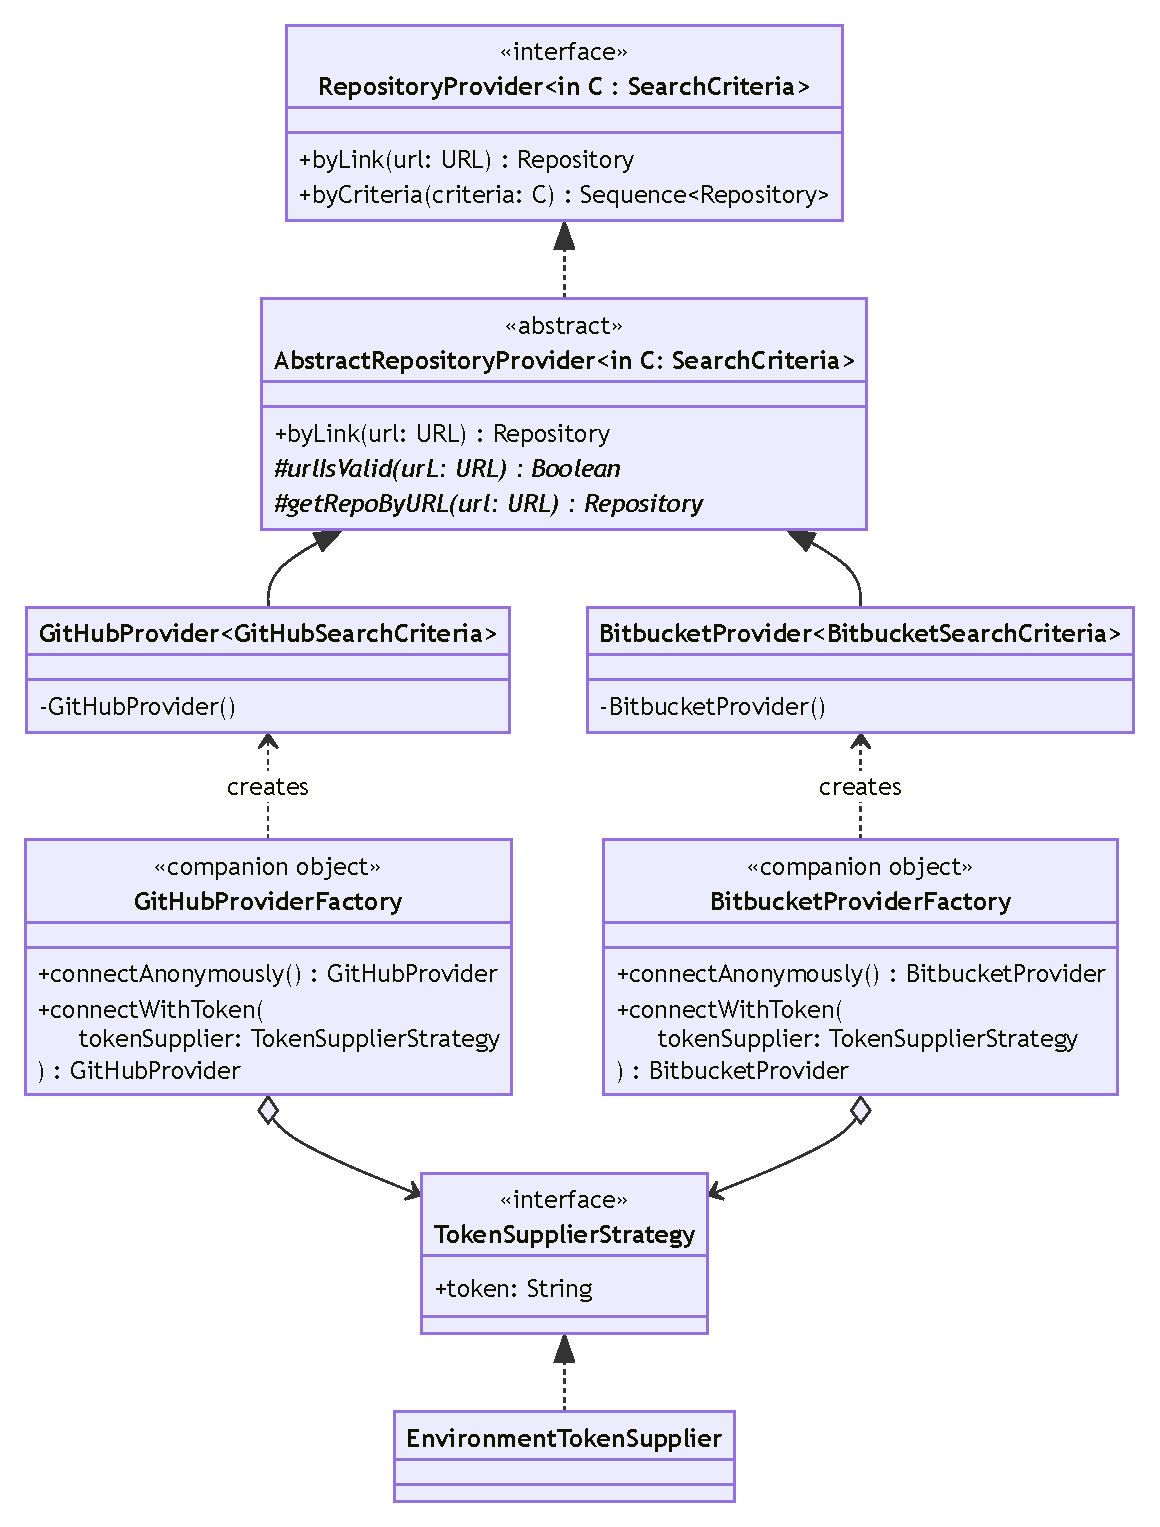
\includegraphics[width=0.9\textwidth]{resources/img/02-provider.pdf}
    \caption{Schema UML dei provider.}
    \label{img:02-provider}
\end{figure}

Viste le limitazioni in termini di numero di richieste che i due servizi impongono \footnote{Sia \textit{GitHub} che \textit{Bitbuckt} hanno un limite massimo di richieste che possono essere effettuate in un certo intervallo di tempo che varia in base la richiesta sia autenticata o meno. Questi vincoli sono imposti per garantire la protezione da attacchi di tipo \textit{Denial of Service}, consentire la scalabilità e garantire buone prestazioni in termini di tempo di risposta.} e la conseguente necessità di autenticarsi mediante degli opportuni \textit{token} per effettuare le richieste \textit{REST}, si è optato di demandare la logica di recupero dei suddetti \textit{token} di autenticazione all'interfaccia \texttt{TokenSupplierStrategy} che reifica il \textit{pattern} \textit{Strategy} \cite{gof}.
%
L'implementazione di \textit{default} ricerca tra variabili d'ambiente, ma altri approcci possono essere introdotti in modo del tutto trasparente ai \textit{provider}.

La creazione dei \textit{provider} avviene per mezzo di due \textit{static factory} \cite{effective-java}, incapsulate all'interno dei due \textit{provider}, in modo da permettere di ottenere un oggetto \textit{provider} anche senza autenticazione.
%
Nonostante questo sia in genere sconsigliato per via delle limitazioni sopra citate, può essere utile in fase di \textit{testing} per permettere di testare il sistema anche in contesti in cui non sia possibile usare \textit{token} di autenticazione validi, ad esempio nel contesto delle \textit{GitHub Actions} nei \textit{workflow} scatenati da eventi di tipo \textit{Pull Request} (vedi...\todo{ref al capitolo implementazione, paragrafo CI})

Dopo una prima analisi delle \textit{API} dei due servizi di \textit{hosting} si è convenuto di permettere di recuperare i progetti mediante due metodi: un \textit{link} diretto alla \textit{repository}, oppure mediante un criterio di ricerca, rappresentato dall'interfaccia \texttt{SearchCriteria}.
%
Per permettere che questi siano componibili è stato qui utilizzato il pattern \textit{Decorator} \cite{gof}.
%
La classe astratta che funge da decoratore è \texttt{(GitHub|BitBucket)CompoundCriteria} e le sue concrete implementazioni permettono di specificare il nome della \textit{repository} o il linguaggio.
%
In questo modo possono essere creati dinamicamente criteri compositi in base alle esigenze del \textit{client} e in futuro potrebbero essere aggiunti nuovi criteri di ricerca, come il numero di stelle ricevute, il \textit{topic} piuttosto che la data di creazione, aderendo all'\textit{Open Closed Principle} secondo cui le entità di un sistema devono essere aperte all'estensione, ma chiuse alla modifica.
%
Il \textit{design} è presentato in \Cref{img:02-search-criteria}.

\begin{sidewaysfigure}
    \centering
    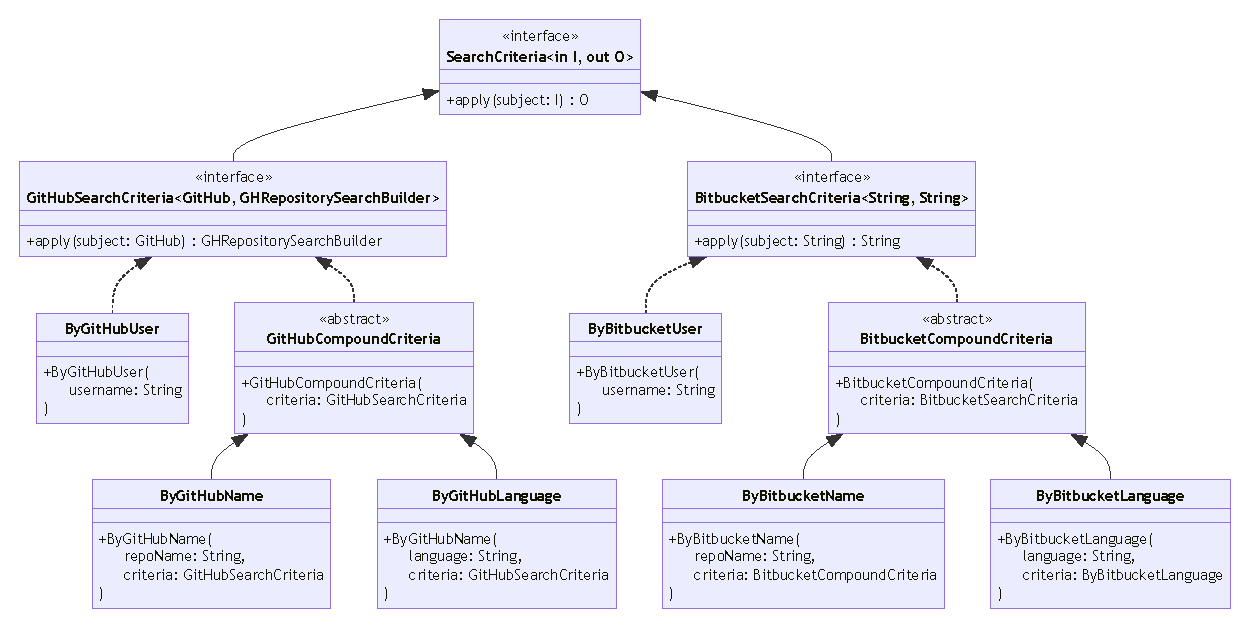
\includegraphics[width=\textwidth]{resources/img/02-search-criteria.pdf}
    \caption{Schema UML dei criteri di ricerca delle \textit{repository}.}
    \label{img:02-search-criteria}
\end{sidewaysfigure}

Le \textit{repository} sono modellate attraverso l'omonima interfaccia, le cui concrete implementazioni rappresentano degli \textit{Adapter} \cite{gof} alle interfacce di libreria utilizzate.
%
Questo permette di essere indipendenti dalla specifica libreria utilizzata, che rimane un dettaglio implementativo, e avere un livello di astrazione adeguato al contesto applicativo.
%
Per quanto attiene la logica del recupero dei sorgenti, in pieno accordo con il \textit{Single Responsability Principle}, è demandata a \texttt{RepoContentSupplierStrategy}.
%
La strategia attualmente in uso consiste nell'effettuare il \textit{clone} della repository in una cartella in locale.

\begin{figure}[h!]
    \makebox[\textwidth][c]{
        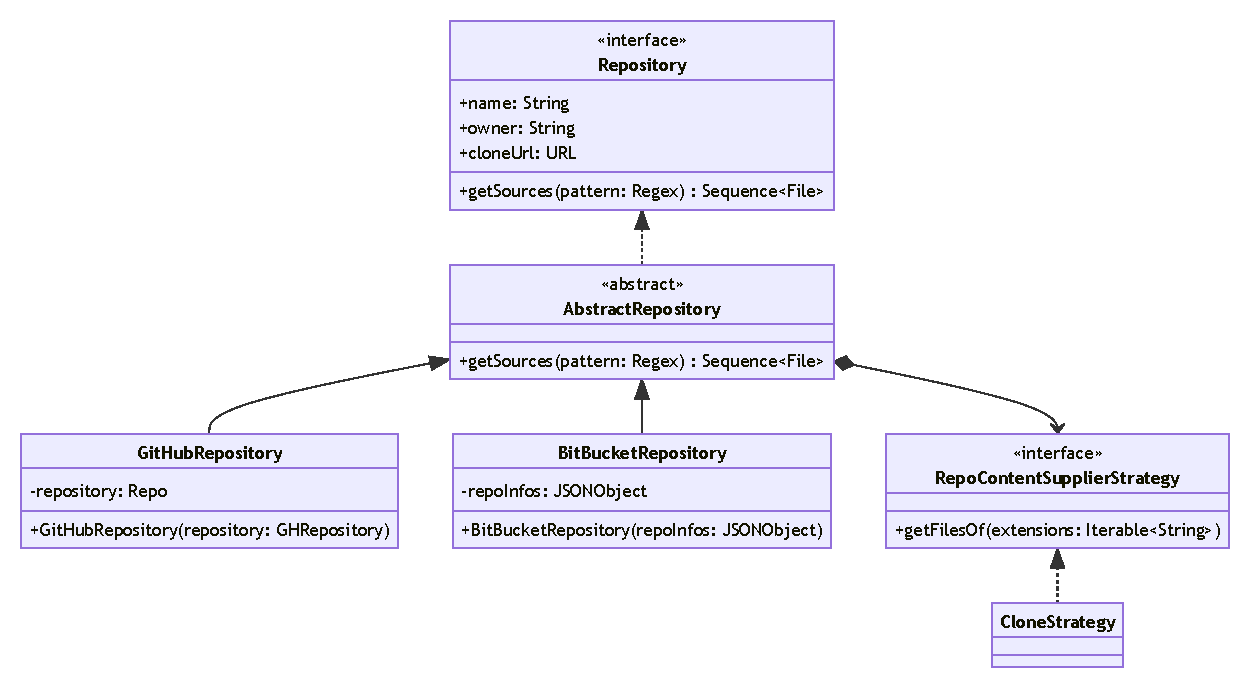
\includegraphics[width=1.2\textwidth]{resources/img/02-repos.pdf}
    }
    \caption{Schema UML delle repository.}
    \label{img:02-repos}
\end{figure}

\subsubsection*{Analizzatore e \textit{detector}}
L'analizzatore, il \textit{filter} e il \textit{detector} sono il cuore dell'intero sistema.
%
Il loro \textit{design} è stato pensato in modo tale da permettere il massimo grado di configurabilità e di estendibilità.
%
Presumibilmente, infatti, questi sono i componenti che varieranno più spesso nell'arco del ciclo di vita di questo \textit{software} e il cui grado di configurabilità influirà certamentente in modo preponderante sia sulle prestazioni, sia sull'efficacia del sistema.

Tutti e tre i componenti sono stati progettati, in stile funzionale, come delle funzioni che, preso i \textit{input} uno più argomenti, ritornano in \textit{output} l'\textit{input} del componente successivo:.
%
L'esecuzione di una tecnica è, infatti, una catena di funzioni applicate in sequenza.

L'analizzatore è il componente che si occupa di trasformare i file sorgenti in rappresentazioni confrontabili.
%
Indipendentemente dalla tipologia di analisi che si voglia applicare, la trasformazione non avviene tramite un semplice passaggio, bensì una sequenza di operazioni che sono eseguite sequenzialmente in cascata.
%
Nel caso in esame, queste sono: il \textit{parsing} del file, una fase di \textit{preprocessing} ed infine la \textit{tokenizzazione} del sorgente.
%
Questa sequenza di azioni è naturalmente modellata attraverso il pattern \textit{Pipeline} \cite{pipeline-pattern}: ogni singolo stadio è modellato attraverso l'interfaccia \texttt{StepHandler} e la \textit{pipeline} viene costruita all'interno del concreto \texttt{Analyzer}, nel nostro caso \texttt{JavaTokenizationAnalyzer}.

\begin{figure}[h!]
    \centering
    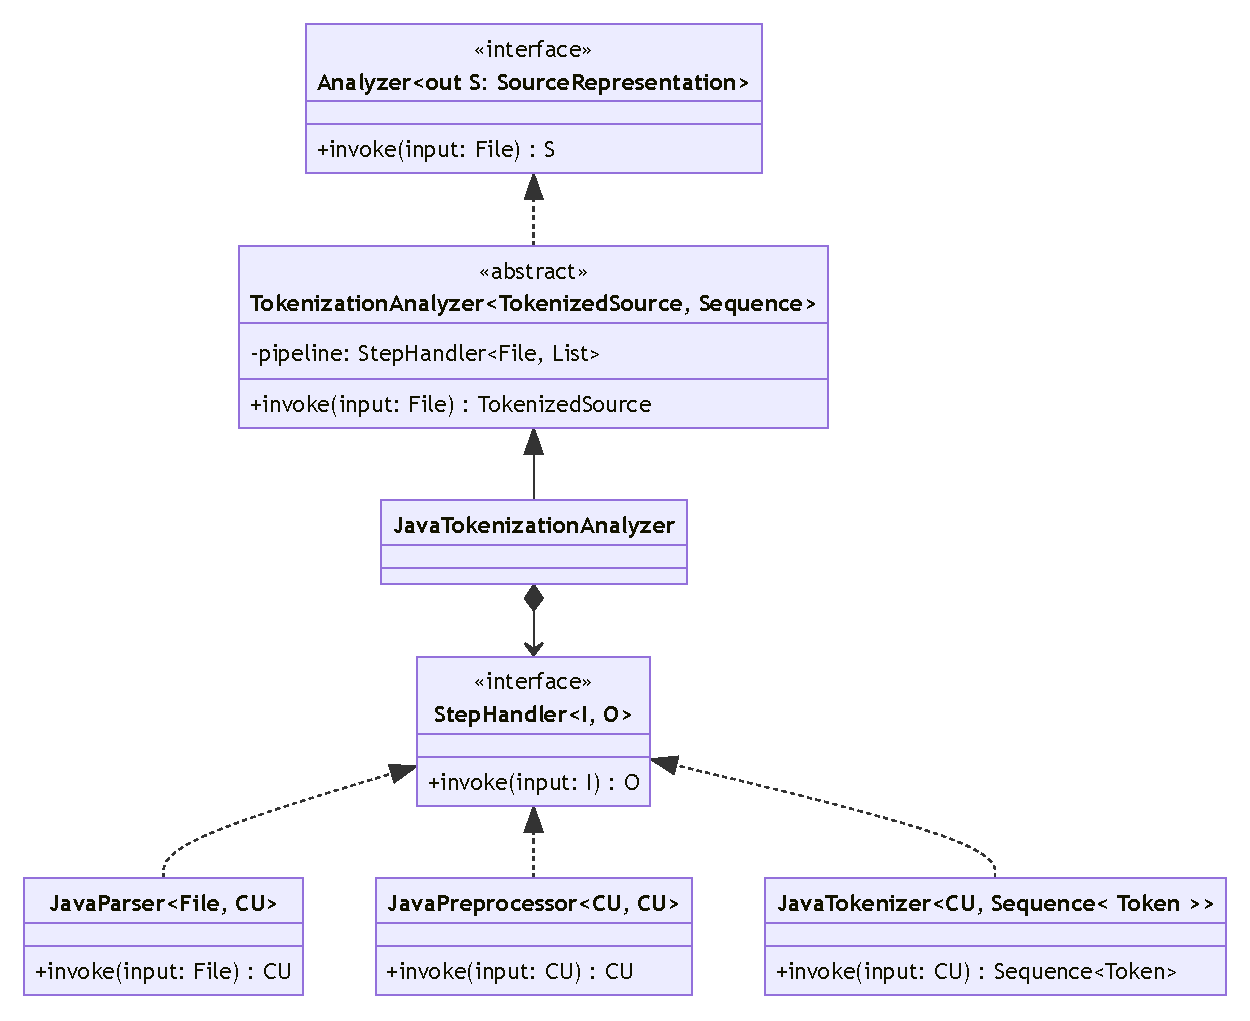
\includegraphics[width=\textwidth]{resources/img/02-analyzer.pdf}
    \caption{Schema UML dell'analizzatore.}
    \label{img:02-analyzer}
\end{figure}

La rappresentazione intermedia prodotta dall'analizzatore è modellata dall'interfaccia \texttt{SourceRepresentation} (\Cref{img:02-representations}). 
%
Tra tutte, quella implementata nell'attuale sistema è composta da una sequenza di \textit{token} e perciò denominata \texttt{TokenizedSource}.
%
L'elenco dei possibili tipi di \textit{token} che la compongono dipende chiaramente dal linguaggio utilizzato.
%
La strategia di recupero di questi ultimi è affidata, al solito tramite \textit{Strategy}, all'interfaccia \texttt{TokenTypesSupplier}, la cui implementazione di \textit{default} effettua la de-serializzazione di un file di configurazione in cui sono salvati tutti le tipologie di \textit{token}.

\begin{figure}[h!]
    \centering
    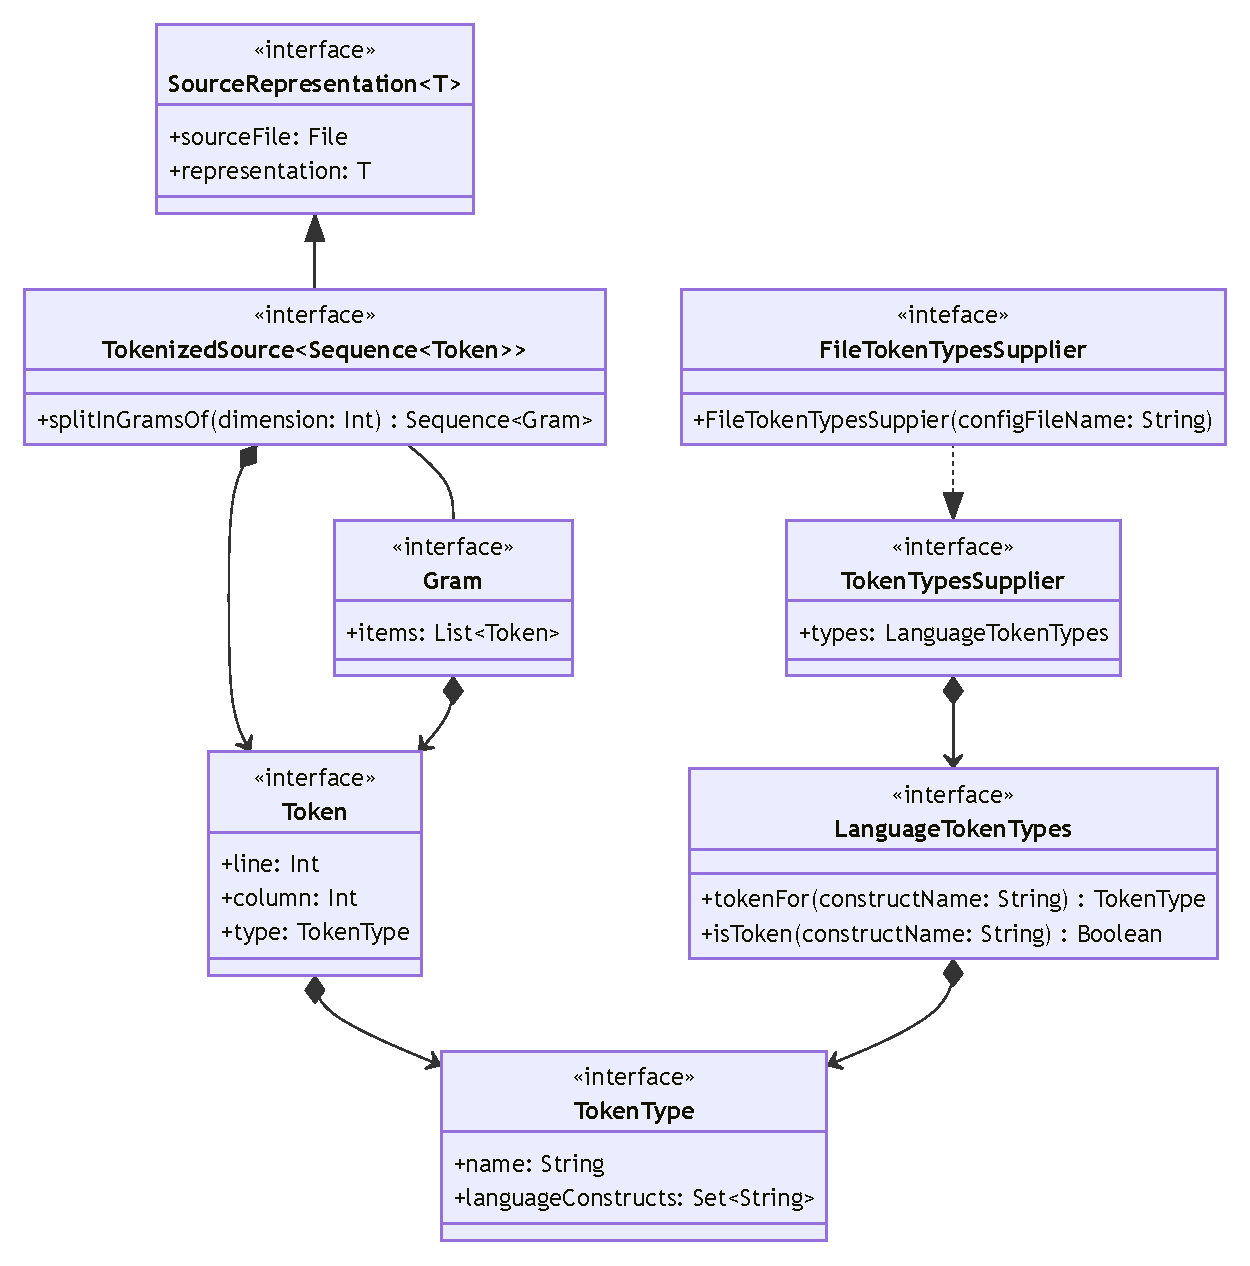
\includegraphics[width=\textwidth]{resources/img/02-representations.pdf}
    \caption{Schema UML delle rappresentazioni intermedie.}
    \label{img:02-representations}
\end{figure}

Le rappresentazioni generate dal processo di analisi, vengono poi opportunamente filtrate per mezzo di un \texttt{RepresentationFilter} che, preso in \textit{input} una istanza dell'insieme delle \textit{submission} e l'insieme del \textit{corpus} con cui confrontarla, ne effettua un filtraggio secondo opportune metriche.
%
Per farlo, fa uso di un \texttt{Indexer} che crea, a partire dalle rappresentazioni, indici (strutture dati) su cui poter effettuare analisi \dots

\todo{filter + schema}

\texttt{PlagiarismDetector} rappresenta invece il componente che individua le similarità tra una coppia di \texttt{SourceRepresentation} e si occupa di calcolare la loro similarità.
%
Poiché vi sono una molteplicità di algoritmi presenti in letteratura che assolvono a questo compito, si è deciso d'implementarli sotto forma di gerarchia di classi di algoritmi il cui contratto comune è definito da \texttt{ComparisonStrategy}. 
%
In particolare, ogni classe implementante \texttt{ComparisonStrategy} genera un \texttt{Match}, dove per \texttt{Match} si intende due sezioni simili di \textit{SourceRepresentation}.
%
L'insieme dei \texttt{Match} che compongono la comparazione di due \texttt{SourceRepresentation} sono raggruppate in un \texttt{ComparisonResult}, il cui grado di similarità è stimato dalla \texttt{SimilarityEstimationStrategy}.

Applicato alla tecnica di \textit{tokenizzazione}, i due concreti algoritmi che implementano la \textit{detection} sono \texttt{Greedy String Tiling} e \texttt{RKRGreedyStringTiling} che ne rappresenta un'estensione più performante.
%
Entrambi generano dei \texttt{TokenMatch}. \dots

\begin{sidewaysfigure}
    \centering
    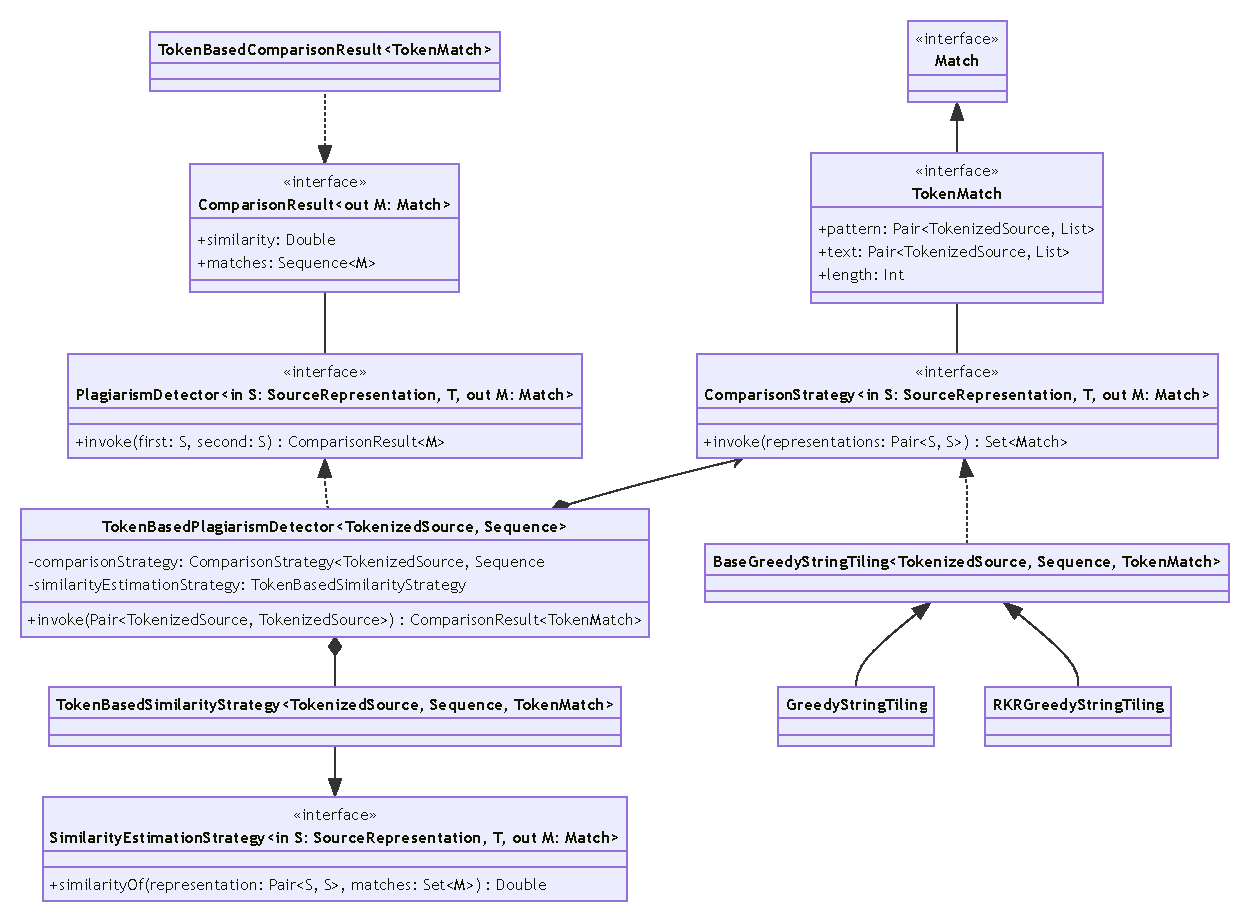
\includegraphics[width=\textwidth]{resources/img/02-detector.pdf}
    \caption{Schema UML del \textit{detector}.}
    \label{img:02-detector}
\end{sidewaysfigure}

Tutti e tre i componenti, \texttt{Analyzer}, \texttt{Filter} e \texttt{PlagiarismDetector}, sono incapsulati all'interno di un concreto \texttt{TechniqueFacade} \cite{gof}.
%
Si è deciso di adottare questo approccio principalmente per due motivi:
\begin{itemize}
    \item la specifiche strategie di analisi e di confronto devono essere istanziate e opportunamente configurate a \textit{runtime} a seconda del tipo di tecnica e delle opzioni scelte dall'utente. Inoltre, devono essere coerenti tra loro: non è possibile, ad esempio, poter istanziare un analizzatore per effettuare la \textit{tokenizzazione} e un rilevatore che non operi sulla sequenza di \textit{token}. Il \textit{facade} pertanto si occupa d'istanziare i corretti componenti necessari all'esecuzione della tecnica in accordo con i parametri a lui fornitogli, sollevando il \textit{client} da questa responsabilità.
    \item Il processo di analisi e confronto può essere complesso. Pertanto si fornisce ai \textit{client} un'interfaccia semplificata che assolve al compito di eseguire una generica tecnica, rendendo di fatto trasparente al chiamante la complessità del sottosistema che, dal suo punto di vista, è di fatto una \textit{black box}.
\end{itemize}

Come già detto, l'aspetto della configurabilità è un aspetto molto importante in questo contesto, in quanto la scelta dei parametri influisce sull'efficacia del rilevamento.
%
In particolare, una specifica sessione è legata ad una particolare configurazione (\texttt{RunConfiguration}) che contiene tutte le informazioni necessarie per l'esecuzione, tra cui la tecnica da utilizzare, l'insieme delle \textit{repository} che compongono la \textit{submission} e quelle del \textit{corpus}, nonché il concreto \texttt{ReportsExporter} a cui è affidata l'esportazione dei \textit{report} generati.
%
Tale configurazione è creata da un concreto \texttt{RunConfigurator}: i due metodi supportati, alternativi tra loro, sono il \texttt{CLIConfigurator} che crea la configurazione a partire dagli argomenti da riga di comando, oppure il \texttt{FileConfigurator} che sfrutta un file di configurazione per impostare tutti i parametri.
%
Nulla vieta che in un prossimo futuro, se si volesse dare una veste grafica al sistema, si possa implementare una interfaccia che specializza \texttt{RunConfigurator} e che viene implementata dalla o dalle classi che si occupano di creare le componenti grafiche.

In \Cref{img:02-session} è mostrato lo schema UML delle classi che mostra i rapporti 

\todo{schema sequenza}

\begin{sidewaysfigure}
    \centering
    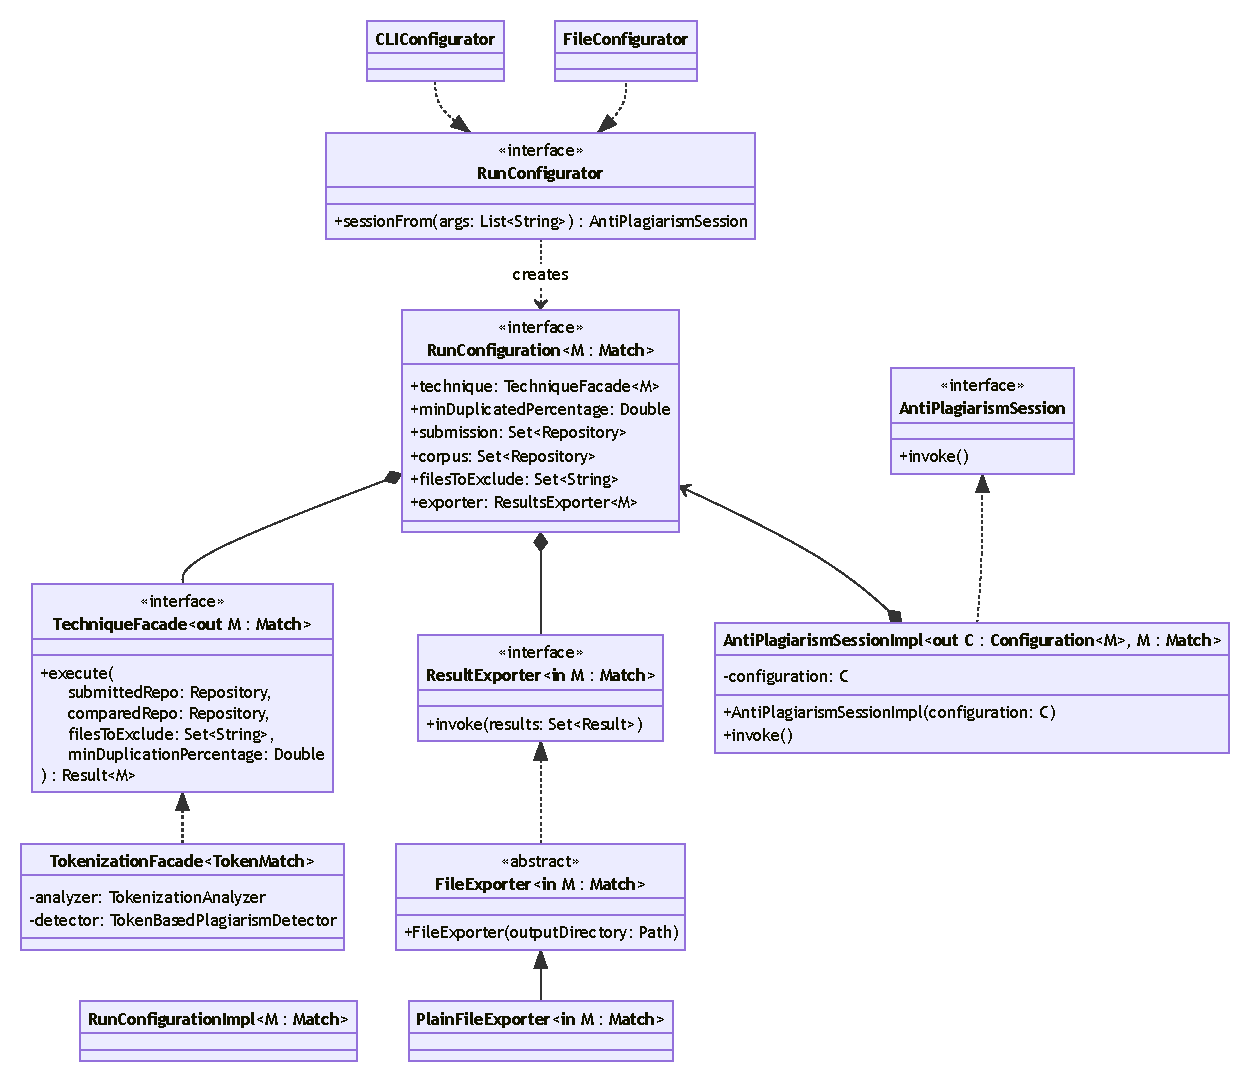
\includegraphics[width=0.9\textheight]{resources/img/02-session.pdf}
    \caption{Schema UML della sessione}
    \label{img:02-session}
\end{sidewaysfigure}

\todo{caching}
